% Options for packages loaded elsewhere
\PassOptionsToPackage{unicode}{hyperref}
\PassOptionsToPackage{hyphens}{url}
%
\documentclass[
  english,
  man, noextraspace]{apa6}
\usepackage{lmodern}
\usepackage{amssymb,amsmath}
\usepackage{ifxetex,ifluatex}
\ifnum 0\ifxetex 1\fi\ifluatex 1\fi=0 % if pdftex
  \usepackage[T1]{fontenc}
  \usepackage[utf8]{inputenc}
  \usepackage{textcomp} % provide euro and other symbols
\else % if luatex or xetex
  \usepackage{unicode-math}
  \defaultfontfeatures{Scale=MatchLowercase}
  \defaultfontfeatures[\rmfamily]{Ligatures=TeX,Scale=1}
\fi
% Use upquote if available, for straight quotes in verbatim environments
\IfFileExists{upquote.sty}{\usepackage{upquote}}{}
\IfFileExists{microtype.sty}{% use microtype if available
  \usepackage[]{microtype}
  \UseMicrotypeSet[protrusion]{basicmath} % disable protrusion for tt fonts
}{}
\makeatletter
\@ifundefined{KOMAClassName}{% if non-KOMA class
  \IfFileExists{parskip.sty}{%
    \usepackage{parskip}
  }{% else
    \setlength{\parindent}{0pt}
    \setlength{\parskip}{6pt plus 2pt minus 1pt}}
}{% if KOMA class
  \KOMAoptions{parskip=half}}
\makeatother
\usepackage{xcolor}
\IfFileExists{xurl.sty}{\usepackage{xurl}}{} % add URL line breaks if available
\IfFileExists{bookmark.sty}{\usepackage{bookmark}}{\usepackage{hyperref}}
\hypersetup{
  pdftitle={COVID-19-Related Institutional Betrayal Among A Sample of Undergraduate Students},
  pdfauthor={Alexis Adams-Clark1,2 \& Jennifer Freyd1,2},
  pdflang={en-EN},
  pdfkeywords={institutional betrayal, institutional courage, trauma symptoms, COVID-19},
  hidelinks,
  pdfcreator={LaTeX via pandoc}}
\urlstyle{same} % disable monospaced font for URLs
\usepackage{graphicx,grffile}
\makeatletter
\def\maxwidth{\ifdim\Gin@nat@width>\linewidth\linewidth\else\Gin@nat@width\fi}
\def\maxheight{\ifdim\Gin@nat@height>\textheight\textheight\else\Gin@nat@height\fi}
\makeatother
% Scale images if necessary, so that they will not overflow the page
% margins by default, and it is still possible to overwrite the defaults
% using explicit options in \includegraphics[width, height, ...]{}
\setkeys{Gin}{width=\maxwidth,height=\maxheight,keepaspectratio}
% Set default figure placement to htbp
\makeatletter
\def\fps@figure{htbp}
\makeatother
\setlength{\emergencystretch}{3em} % prevent overfull lines
\providecommand{\tightlist}{%
  \setlength{\itemsep}{0pt}\setlength{\parskip}{0pt}}
\setcounter{secnumdepth}{-\maxdimen} % remove section numbering
% Make \paragraph and \subparagraph free-standing
\ifx\paragraph\undefined\else
  \let\oldparagraph\paragraph
  \renewcommand{\paragraph}[1]{\oldparagraph{#1}\mbox{}}
\fi
\ifx\subparagraph\undefined\else
  \let\oldsubparagraph\subparagraph
  \renewcommand{\subparagraph}[1]{\oldsubparagraph{#1}\mbox{}}
\fi
% Manuscript styling
\usepackage{upgreek}
\captionsetup{font=singlespacing,justification=justified}

% Table formatting
\usepackage{longtable}
\usepackage{lscape}
% \usepackage[counterclockwise]{rotating}   % Landscape page setup for large tables
\usepackage{multirow}		% Table styling
\usepackage{tabularx}		% Control Column width
\usepackage[flushleft]{threeparttable}	% Allows for three part tables with a specified notes section
\usepackage{threeparttablex}            % Lets threeparttable work with longtable

% Create new environments so endfloat can handle them
% \newenvironment{ltable}
%   {\begin{landscape}\begin{center}\begin{threeparttable}}
%   {\end{threeparttable}\end{center}\end{landscape}}
\newenvironment{lltable}{\begin{landscape}\begin{center}\begin{ThreePartTable}}{\end{ThreePartTable}\end{center}\end{landscape}}

% Enables adjusting longtable caption width to table width
% Solution found at http://golatex.de/longtable-mit-caption-so-breit-wie-die-tabelle-t15767.html
\makeatletter
\newcommand\LastLTentrywidth{1em}
\newlength\longtablewidth
\setlength{\longtablewidth}{1in}
\newcommand{\getlongtablewidth}{\begingroup \ifcsname LT@\roman{LT@tables}\endcsname \global\longtablewidth=0pt \renewcommand{\LT@entry}[2]{\global\advance\longtablewidth by ##2\relax\gdef\LastLTentrywidth{##2}}\@nameuse{LT@\roman{LT@tables}} \fi \endgroup}

% \setlength{\parindent}{0.5in}
% \setlength{\parskip}{0pt plus 0pt minus 0pt}

% \usepackage{etoolbox}
\makeatletter
\patchcmd{\HyOrg@maketitle}
  {\section{\normalfont\normalsize\abstractname}}
  {\section*{\normalfont\normalsize\abstractname}}
  {}{\typeout{Failed to patch abstract.}}
\patchcmd{\HyOrg@maketitle}
  {\section{\protect\normalfont{\@title}}}
  {\section*{\protect\normalfont{\@title}}}
  {}{\typeout{Failed to patch title.}}
\makeatother
\shorttitle{COVID-19 Institutional Betrayal}
\keywords{institutional betrayal, institutional courage, trauma symptoms, COVID-19\newline\indent Word count: X}
\DeclareDelayedFloatFlavor{ThreePartTable}{table}
\DeclareDelayedFloatFlavor{lltable}{table}
\DeclareDelayedFloatFlavor*{longtable}{table}
\makeatletter
\renewcommand{\efloat@iwrite}[1]{\immediate\expandafter\protected@write\csname efloat@post#1\endcsname{}}
\makeatother
\usepackage{lineno}

\linenumbers
\usepackage{csquotes}
\ifxetex
  % Load polyglossia as late as possible: uses bidi with RTL langages (e.g. Hebrew, Arabic)
  \usepackage{polyglossia}
  \setmainlanguage[]{english}
\else
  \usepackage[shorthands=off,main=english]{babel}
\fi

\title{\textbf{COVID-19-Related Institutional Betrayal Among A Sample of Undergraduate Students}}
\author{Alexis Adams-Clark\textsuperscript{1,2} \& Jennifer Freyd\textsuperscript{1,2}}
\date{}


\authornote{

University of Oregon, Department of Psychology, 1227 University St.~Eugene, OR 97401
Center for Institutional Courage, Inc., Palo Alto, CA

The authors made the following contributions. Alexis Adams-Clark: Conceptualization, Writing - Original Draft Preparation, Writing - Review \& Editing; Jennifer Freyd: Conceptualization, Writing - Review \& Editing.

Correspondence concerning this article should be addressed to Alexis Adams-Clark, 1227 University St.~Eugene, OR 97401. E-mail: \href{mailto:aadamscl@uoregon.edu}{\nolinkurl{aadamscl@uoregon.edu}}

}

\affiliation{\vspace{0.5cm}\textsuperscript{1} University of Oregon\\\textsuperscript{2} Center for Institutional Courage}

\abstract{
Individuals are dependent on institutions (e.g., universities, governments, healthcare systems) to protect their safety and advocate for their needs. When institutions harm the individuals who depend on them, they commit \emph{institutional betrayal}, which has been associated with numerous negative outcomes. Throughout the COVID-19 pandemic, students have put entrusted universities to protect both their health and their educational opportunities. However, many universities have failed to meet these expectations, and it is likely that many students experience a sense of COVID-19-related institutional betrayal. The current study examined the prevalence and correlates of institutional betrayal among a sample of 309 undergraduate students at a large, public university in the Northwest United States. Results revealed that 66\% of students endorsed at least one type of COVID-19-related institutional betrayal. Higher institutional betrayal ratings were significantly correlated with both current general trauma related symptoms, \emph{r} = .21, \emph{p} \textless{} .001, and COVID-19-related trauma symptoms, \emph{r} = .22, \emph{p} \textless{} .001. These results suggest that COVID-19 institutional betrayal is common and may be associated with distress among undergraduate students.
}



\begin{document}
\maketitle

\raggedbottom
\centering

\textbf{\enquote{In the absence of any national strategy for tackling the coronavirus pandemic, colleges and universities in the United States are on their own when it comes to deciding whether and how to bring students back for the autumn term, which has already started for some institutions. Many are relying on their own experts, resulting in a wide range of approaches\ldots It all amounts to a gigantic, unorganized public-health experiment --- with millions of students and an untold number of faculty members and staff as participants.} (Marris, 2020)}

\raggedright

\setlength{\parindent}{5ex}

Individuals are frequently dependent on societal institutions (e.g., universities, governments, healthcare systems) to protect their safety, provide them with vital services, and advocate for their needs. There are few times in recent history when this has been more true than during the coronavirus pandemic; in such a time of crisis, individuals turned to various institutions to enact and enforce policies to curb the spread of COVID-19, mobilize efforts to create treatments and vaccines, and equitably distribute care to those infected. However, in multiple domains, institutional efforts were left wanting, as COVID-19 infections continue to proliferate.

The term \emph{institutional betrayal} (Smith \& Freyd, 2014) can be used to describe such an occurrence. Institutional betrayal manifests when a institution fails to fulfill its obligations to institutional members who entrust and depend upon it. Such a betrayal can occur through both institutional actions (e.g., an institution actively committing a transgression or violation against a member) or inactions (e.g., an institution failing to enact appropriate policies or respond adequately to an expressed concern). In past research, institutional betrayal has largely been studied in the context of campus sexual assault (Smith \& Freyd, 2013), healthcare experiences (Carly Parnitzke Smith, 2017), and military sexual trauma (Monteith, Bahraini, Matarazzo, Soberay, \& Smith, 2016), but it may also apply to a range of experiences throughout the COVID-19 pandemic.

Although scholars have identified several instances of institutional betrayal occurring as throughout the COVID-19 pandemic, such as betrayal by healthcare systems (Klest, Smith, May, McCall-Hosenfeld, \& Tamaian, 2020) and by government leaders (DePrince \& Cook, 2020), less commentary exists regarding possible experiences of institutional betrayal by college students in the context of their university institution. Throughout the COVID-19 pandemic, students have entrusted, and at times forcibly made to rely on, universities to protect both their health and educational opportunities, even as COVID-19 cases rise on many campuses (Lu et al., 2020). Although many universities, including the authors' own institution, have enacted numerous policies that aim to curb the spread of COVID-19 (e.g., mask mandates, frequent cleaning), many have also have simultaneously created situations in which COVID-19 transmission is more likely (e.g., holding some in-person classes, requiring first-year students to live in on-campus dormitories), which have lead to rising rates of infection on campuses. Even those students at universities that have implemented strict, remote-only instruction, may experience a sense of institutional betrayal regarding challenges related to remote learning, which are exacerbated further by existing inequities.

Covid-19-related institutional betrayal among college students is particularly important to acknowledge and measure, given that prior research suggests that specific harm is created when trusted institutions fail to fulfill promises. Experiences of institutional betrayal in other contexts have been found to be associated with numerous negative mental health outcomes, including trauma-related symptoms (Lind, Adams-Clark, \& Freyd, 2020; Smith \& Freyd, 2013), physical health outcomes (Carly P Smith \& Freyd, 2017), suicidal ideation (Monteith et al., 2016), and disengagement from healthcare services (Carly Parnitzke Smith, 2017). If students are experiencing COVID-19-related institutional betrayal, they may be also be experiencing similar outcomes, which likely affect students' academic engagement.

The current study seeks to describe and characterize the prevalence of students' experiences of COVID-19-related institutional betrayal. Using a sample of undergraduate students, we measured the incidence rate of 12 types of COVID-19-related institutional betrayal, as well as initial associations between institutional betrayal and students' self-reported general trauma-related symptoms, COVID-19 specific trauma-related symptoms, and degree of identification with (i.e., feeling \enquote{a part of}) the university as a whole. (\emph{Note: I'll be adding a second sample for a Study 2 section, but data isn't done being collected}). In this study, we had the following hypotheses:

\begin{enumerate}
\def\labelenumi{\arabic{enumi}.}
\item
  A significant portion of students would report experiencing COVID-19-related institutional betrayal.
\item
  Experiences of institutional betrayal would be related to both general and COVID-19 specific trauma-related symptoms. The relationship between institutional betrayal and COVID-19 specific trauma symptoms would persist, even when controlling for demographic factors and general symptoms.
\item
  Students overall would report less identification with the university since COVID-19 (compared to a retrospective report of how they felt prior to COVID-19), and this decrease would be moderated by institutional betrayal, such that those experiencing high rates of institutional betrayal would report the greatest decrease in identification.
\end{enumerate}

\setlength{\parindent}{5ex}

\hypertarget{method}{%
\section{Method}\label{method}}

\hypertarget{participants}{%
\subsection{Participants}\label{participants}}

Participants were recruited from the Human Subjects Pool at a large, public university in the Northwest United States. The university's Human Subjects Pool contains undergraduate students currently enrolled in introductory psychology and linguistics courses, and these students receive course credit for their participation in research studies. Students are not aware of the topic of any given study prior to signing up, which reduces self-selection bias (although they do have the option to end participation during the informed consent process or at any time throughout the study). A total of 346 undergraduate students signed up and consented to participate in the present study. Participants who failed to correctly answer at least four out of five \enquote{attention check} questions randomly located throughout the survey (e.g.~"please choose \enquote{strongly agree} if you are paying attention) were removed prior to data analysis (n = 37). The final sample used for data analysis consisted of 309 participants (71.5\% women, 26.5\% men, 1.9\% non-binary/gender-nonconforming). The majority of participants were White (63.4\%), and the average age of participants was 19.39 (SD = 1.45), and first-year (44.3\%) or second-year (29.4\%) students.

These data were collected during the fall 2020 term of the academic year, during which COVID-19 infections were steadily climbing at the university, local, and national level. The university at the focus of the current investigation adopted a largely remote learning environment. However, the university required all first-year students to live in dormitories on campus, and a minority of classes were held in person.

\hypertarget{measures}{%
\subsection{Measures}\label{measures}}

\textbf{COVID-19-Related Institutional Betrayal}. COVID-19-related institutional betrayal was measured using an adapted version of the Institutional Betrayal Questionnaire (IBQ; (Smith \& Freyd, 2013, p. @smith2017). The IBQ consists of 12 items listing actions or inactions by an institution in rsponse to a traumatic event, and it has been established as a valid measure of institutional betrayal. Although originally designed to assess the university's responses to instances of sexual violence, the measure was adapted to apply to the university's responses to the COVID-19 pandemic. Participants were instructed to answer each item (e.g., \enquote{did your university create an environment in which COVID-19 infection and safety violations seemed more likely?}) by selecting \enquote{Yes,} \enquote{No,} or \enquote{Not Applicable.} \enquote{Yes} responses were coded as 1 and were summed to create a total IBQ score ranging from 0 to 12. The distribution was skewed (1.38) and kurtotic (1.31), but within the range in which the assumption of normality can be maintained without transformation. At the end of the scale, students were asked to rate the extent to which they identified with the institution both prior to and since the COVID-19 pandemic.

\textbf{Trauma-related symptoms.} General trauma-related symptoms were measured using the Trauma Symptoms Checklist (Elliott \& Briere, 1992), which is a valid, standard measure of various symptoms that may be related to traumatic experiences. The scale consists of several subscales, including Dissociation subscale, Sleep Disturbance subscale, Sexual Problems subscale, Anxiety subscale, Depression subscale, and the Sexual Abuse Trauma Index subscale. For the present study, only the total overall TSC score was used for analysis, and items were summed and averaged to create an \enquote{average} TSC score for each participant. Participants were asked to rate the frequency of various symptoms in the past two months, using the anchors ranging from 0 (\enquote{Never}) to 3 (\enquote{Often}). The scale demonstrated satisfactory reliability in this current study (alpha = .94).

\textbf{COVID-19-specific trauma cognitions.} COVID-19-specific trauma cognitions were measured using an adapted version of the Impact of Events Scale (IES; (Horowitz, Wilner, \& Alvarez, 1979) that has been adapted to COVID-19 (ref). This scale specifically measures avoidance and intrusion cognitions related to COVID-19. Avoidance and intrusive symptoms often occur following exposure to a specific traumatic event. Participants were asked to rate the frequency of each symptom (e.g., \enquote{I had trouble falling asleep because thoughts about COVID-19 came into my mind}) in the past week, using anchors ranging from 0 (\enquote{Never}) to 3 (\enquote{Often}). Items were summed and averaged to create an \enquote{average} IES score for each participant. The scale demonstrated satisfactory reliability in this current study (alpha = .90).

\hypertarget{procedure}{%
\subsection{Procedure}\label{procedure}}

In the present study, all participants reviewed an informed consent form before participation. After consenting to participate, participants completed questionnaires through an online survey hosted on \emph{Qualtrics} from a personal electronic device in a private location of their choosing. Participants had the option to leave items blank and to discontinue participation at any time. Upon completion of the survey, participants reviewed a debriefing form and received course credit for their participation. All study procedures were approved by the university's Office of Research Compliance (Institutional Review Board).

\hypertarget{data-analysis}{%
\subsection{Data analysis}\label{data-analysis}}

We used R (Version 4.0.2; R Core Team, 2020) and the R-packages \emph{apaTables} (Version 2.0.5; Stanley, 2018), \emph{corx} (Version 1.0.6.1; Conigrave, 2020), \emph{dplyr} (Version 1.0.4; Wickham, François, Henry, \& Müller, 2021), \emph{forcats} (Version 0.5.0; Wickham, 2020a), \emph{ggplot2} (Version 3.3.2; Wickham, 2016), \emph{here} (Version 0.1; Müller, 2017), \emph{papaja} (Version 0.1.0.9997; Aust \& Barth, 2020), \emph{psych} (Version 2.0.7; Revelle, 2020), \emph{purrr} (Version 0.3.4; Henry \& Wickham, 2020), \emph{readr} (Version 1.3.1; Wickham, Hester, \& Francois, 2018), \emph{rio} (Version 0.5.16; Chan, Chan, Leeper, \& Becker, 2018), \emph{skimr} (Version 2.1.2; Waring et al., 2020), \emph{stringr} (Version 1.4.0; Wickham, 2019), \emph{tibble} (Version 3.0.6; Müller \& Wickham, 2021), \emph{tidyr} (Version 1.1.2; Wickham, 2020b), and \emph{tidyverse} (Version 1.3.0; Wickham et al., 2019) for all our analyses.

\hypertarget{results}{%
\section{Results}\label{results}}

\begin{figure}[H]

{\centering 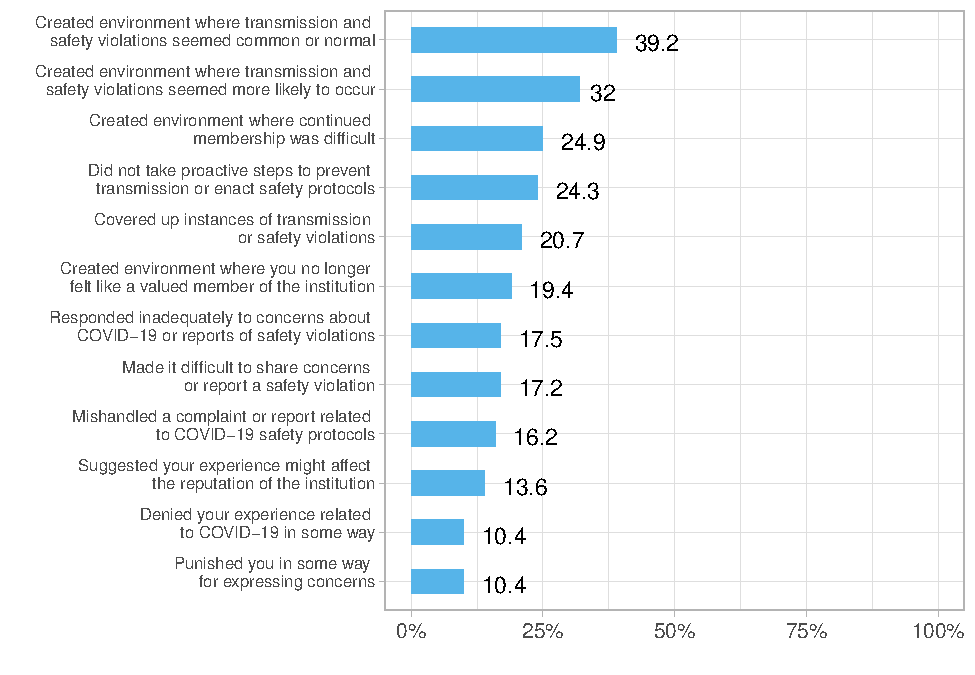
\includegraphics[width=\textwidth]{papaja_doc_files/figure-latex/figure1-1} 

}

\caption{Percentage of Students Endorsing Institutional Betrayal
}\label{fig:figure1}
\end{figure}

\begin{figure}[H]

{\centering 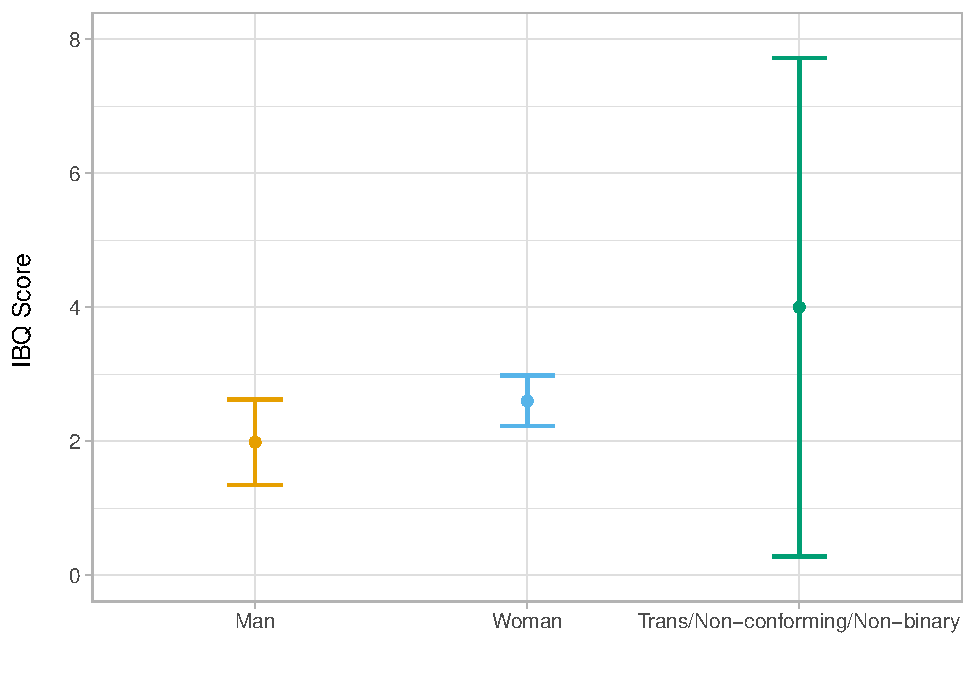
\includegraphics[width=\textwidth]{papaja_doc_files/figure-latex/figure2-1} 

}

\caption{Institutional Betrayal Score by Gender (N = 309) 
}\label{fig:figure2}
\end{figure}

The majority of students (66.34\%) reported at least one type of COVID-19-related institutional betrayal. The most common types of institutional betrayal reported were \enquote{creating an environment in which COVID-19 transmission was more common or seemed normal} and \enquote{failure to prevent COVID-19 transmission} (See Figure \ref{fig:figure1}). There were no significant differences in COVID-19-related institutional betrayal by gender (See Figure \ref{fig:figure2}).

\begin{table}[tbp]

\begin{center}
\begin{threeparttable}

\caption{\label{tab:table1}Example corr matrix}

\begin{tabular}{lllll}
\toprule
 & \multicolumn{1}{c}{1} & \multicolumn{1}{c}{2} & \multicolumn{1}{c}{$M$} & \multicolumn{1}{c}{$SD$}\\
\midrule
1. Institutional Betrayal Score & - &  & 2.47 & 2.90\\
2. Trauma Symptom Score & .22*** & - & 0.87 & 0.53\\
3. Impact of Event Score & .21*** & .44*** & 1.07 & 0.64\\
\bottomrule
\addlinespace
\end{tabular}

\begin{tablenotes}[para]
\normalsize{\textit{Note.} * p < 0.05; ** p < 0.01; *** p < 0.001}
\end{tablenotes}

\end{threeparttable}
\end{center}

\end{table}

\begin{table}[tbp]

\begin{center}
\begin{threeparttable}

\caption{\label{tab:table2}A full regression table.}

\begin{tabular}{lllll}
\toprule
Predictor & \multicolumn{1}{c}{$b$} & \multicolumn{1}{c}{95\% CI} & \multicolumn{1}{c}{$t(276)$} & \multicolumn{1}{c}{$p$}\\
\midrule
Intercept & 0.33 & $[0.16$, $0.50]$ & 3.78 & < .001\\
GenderWoman & 0.19 & $[0.04$, $0.34]$ & 2.54 & .012\\
GenderTrans/Non-conforming/Non-binary & 0.33 & $[-0.13$, $0.79]$ & 1.43 & .154\\
Covid19know someone with covid & 0.21 & $[0.07$, $0.35]$ & 3.00 & .003\\
Tsc mean & 0.40 & $[0.27$, $0.53]$ & 6.18 & < .001\\
Ibq sum & 0.03 & $[0.00$, $0.05]$ & 2.39 & .017\\
\bottomrule
\addlinespace
\end{tabular}

\begin{tablenotes}[para]
\normalsize{\textit{Note.} * p < 0.05; ** p < 0.01; *** p < 0.001}
\end{tablenotes}

\end{threeparttable}
\end{center}

\end{table}

Institutional betrayal was significantly associated with both general trauma-related symptoms and COVID-19 specific avoidance and intrusion symptoms, \emph{p} \textless{} .001 (see Table \ref{tab:table1}). Institutional betrayal was associated with unique variance in COVID-19 specific avoidance and intrusion symptoms, \emph{p} = .01 (see Table \ref{tab:table2}), even when controlling for gender, knowing someone close with COVID-19, and non-specific trauma-related distress.

\begin{figure}[H]

{\centering 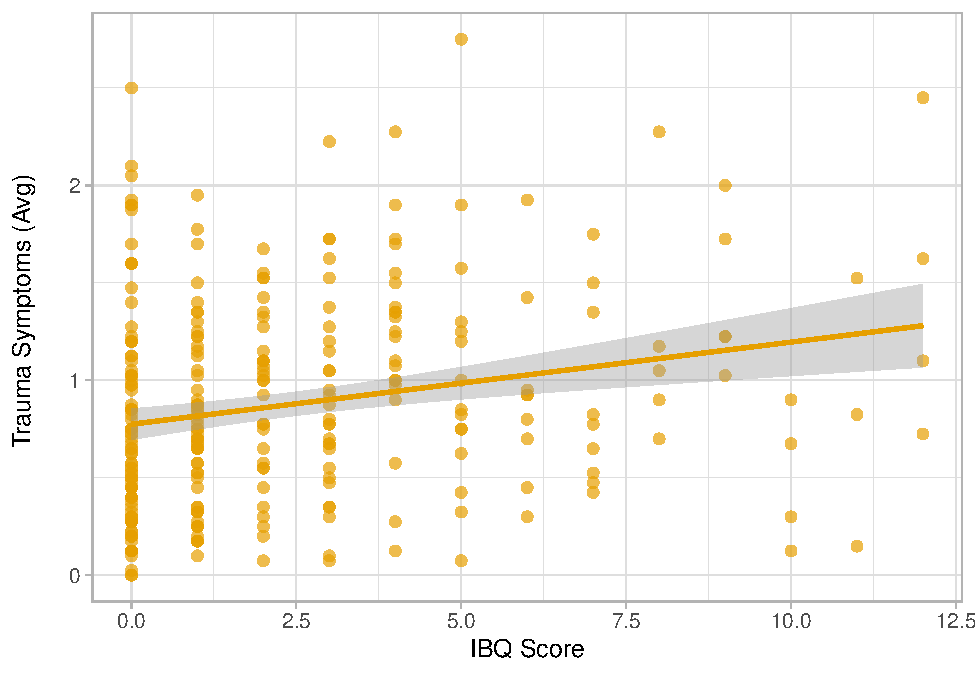
\includegraphics[width=\textwidth]{papaja_doc_files/figure-latex/figure3-1} 

}

\caption{Institutional Identity by Institutional Betrayal (N = 309) 
}\label{fig:figure3}
\end{figure}

\begin{table}[tbp]

\begin{center}
\begin{threeparttable}

\caption{\label{tab:table3}A full regression table.}

\begin{tabular}{lllll}
\toprule
Predictor & \multicolumn{1}{c}{$b$} & \multicolumn{1}{c}{95\% CI} & \multicolumn{1}{c}{$t(301)$} & \multicolumn{1}{c}{$p$}\\
\midrule
Intercept & 0.07 & $[-0.08$, $0.21]$ & 0.89 & .377\\
Scaleid 1before & 0.21 & $[0.06$, $0.35]$ & 2.79 & .006\\
Ibq sum & -0.02 & $[-0.06$, $0.02]$ & -0.86 & .390\\
Scaleid 1before $\times$ Ibq sum & -0.06 & $[-0.10$, $-0.02]$ & -2.86 & .005\\
\bottomrule
\addlinespace
\end{tabular}

\begin{tablenotes}[para]
\normalsize{\textit{Note.} * p < 0.05; ** p < 0.01; *** p < 0.001}
\end{tablenotes}

\end{threeparttable}
\end{center}

\end{table}

\hypertarget{discussion}{%
\section{Discussion}\label{discussion}}

\newpage

\hypertarget{references}{%
\section{References}\label{references}}

\begingroup
\setlength{\parindent}{-0.5in}
\setlength{\leftskip}{0.5in}

\hypertarget{refs}{}
\leavevmode\hypertarget{ref-R-papaja}{}%
Aust, F., \& Barth, M. (2020). \emph{papaja: Create APA manuscripts with R Markdown}. Retrieved from \url{https://github.com/crsh/papaja}

\leavevmode\hypertarget{ref-R-rio}{}%
Chan, C.-h., Chan, G. C., Leeper, T. J., \& Becker, J. (2018). \emph{Rio: A swiss-army knife for data file i/o}.

\leavevmode\hypertarget{ref-R-corx}{}%
Conigrave, J. (2020). \emph{Corx: Create and format correlation matrices}. Retrieved from \url{https://CRAN.R-project.org/package=corx}

\leavevmode\hypertarget{ref-elliott1992}{}%
Elliott, D. M., \& Briere, J. (1992). Sexual abuse trauma among professional women: Validating the trauma symptom checklist-40 (tsc-40). \emph{Child Abuse \& Neglect}, \emph{16}(3), 391--398.

\leavevmode\hypertarget{ref-R-purrr}{}%
Henry, L., \& Wickham, H. (2020). \emph{Purrr: Functional programming tools}. Retrieved from \url{https://CRAN.R-project.org/package=purrr}

\leavevmode\hypertarget{ref-horowitz1979}{}%
Horowitz, M., Wilner, N., \& Alvarez, W. (1979). Impact of event scale: A measure of subjective stress. \emph{Psychosomatic Medicine}, \emph{41}(3), 209--218.

\leavevmode\hypertarget{ref-klest2020}{}%
Klest, B., Smith, C. P., May, C., McCall-Hosenfeld, J., \& Tamaian, A. (2020). COVID-19 has united patients and providers against institutional betrayal in health care: A battle to be heard, believed, and protected. \emph{Psychological Trauma: Theory, Research, Practice, and Policy}, \emph{12}(S1), S159.

\leavevmode\hypertarget{ref-lind2020}{}%
Lind, M. N., Adams-Clark, A. A., \& Freyd, J. J. (2020). Isn't high school bad enough already? Rates of gender harassment and institutional betrayal in high school and their association with trauma-related symptoms. \emph{PloS One}, \emph{15}(8), e0237713.

\leavevmode\hypertarget{ref-lu2020college}{}%
Lu, H., Weintz, C., Pace, J., Indana, D., Linka, K., \& Kuhl, E. (2020). Are college campuses superspreaders? A data-driven modeling study. \emph{Computer Methods in Biomechanics and Biomedical Engineering}, 1--11.

\leavevmode\hypertarget{ref-monteith2016}{}%
Monteith, L. L., Bahraini, N. H., Matarazzo, B. B., Soberay, K. A., \& Smith, C. P. (2016). Perceptions of institutional betrayal predict suicidal self-directed violence among veterans exposed to military sexual trauma. \emph{Journal of Clinical Psychology}, \emph{72}(7), 743--755.

\leavevmode\hypertarget{ref-R-here}{}%
Müller, K. (2017). \emph{Here: A simpler way to find your files}. Retrieved from \url{https://CRAN.R-project.org/package=here}

\leavevmode\hypertarget{ref-R-tibble}{}%
Müller, K., \& Wickham, H. (2021). \emph{Tibble: Simple data frames}. Retrieved from \url{https://CRAN.R-project.org/package=tibble}

\leavevmode\hypertarget{ref-R-base}{}%
R Core Team. (2020). \emph{R: A language and environment for statistical computing}. Vienna, Austria: R Foundation for Statistical Computing. Retrieved from \url{https://www.R-project.org/}

\leavevmode\hypertarget{ref-R-psych}{}%
Revelle, W. (2020). \emph{Psych: Procedures for psychological, psychometric, and personality research}. Evanston, Illinois: Northwestern University. Retrieved from \url{https://CRAN.R-project.org/package=psych}

\leavevmode\hypertarget{ref-smith2017first}{}%
Smith, C. P. (2017). First, do no harm: Institutional betrayal and trust in health care organizations. \emph{Journal of Multidisciplinary Healthcare}, \emph{10}, 133.

\leavevmode\hypertarget{ref-smith2013}{}%
Smith, C. P., \& Freyd, J. J. (2013). Dangerous safe havens: Institutional betrayal exacerbates sexual trauma. \emph{Journal of Traumatic Stress}, \emph{26}(1), 119--124.

\leavevmode\hypertarget{ref-smith2014}{}%
Smith, C. P., \& Freyd, J. J. (2014). Institutional betrayal. \emph{American Psychologist}, \emph{69}(6), 575.

\leavevmode\hypertarget{ref-smith2017}{}%
Smith, C. P., \& Freyd, J. J. (2017). Insult, then injury: Interpersonal and institutional betrayal linked to health and dissociation. \emph{Journal of Aggression, Maltreatment \& Trauma}, \emph{26}(10), 1117--1131.

\leavevmode\hypertarget{ref-R-apaTables}{}%
Stanley, D. (2018). \emph{ApaTables: Create american psychological association (apa) style tables}. Retrieved from \url{https://CRAN.R-project.org/package=apaTables}

\leavevmode\hypertarget{ref-R-skimr}{}%
Waring, E., Quinn, M., McNamara, A., Arino de la Rubia, E., Zhu, H., \& Ellis, S. (2020). \emph{Skimr: Compact and flexible summaries of data}. Retrieved from \url{https://CRAN.R-project.org/package=skimr}

\leavevmode\hypertarget{ref-R-ggplot2}{}%
Wickham, H. (2016). \emph{Ggplot2: Elegant graphics for data analysis}. Springer-Verlag New York. Retrieved from \url{https://ggplot2.tidyverse.org}

\leavevmode\hypertarget{ref-R-stringr}{}%
Wickham, H. (2019). \emph{Stringr: Simple, consistent wrappers for common string operations}. Retrieved from \url{https://CRAN.R-project.org/package=stringr}

\leavevmode\hypertarget{ref-R-forcats}{}%
Wickham, H. (2020a). \emph{Forcats: Tools for working with categorical variables (factors)}. Retrieved from \url{https://CRAN.R-project.org/package=forcats}

\leavevmode\hypertarget{ref-R-tidyr}{}%
Wickham, H. (2020b). \emph{Tidyr: Tidy messy data}. Retrieved from \url{https://CRAN.R-project.org/package=tidyr}

\leavevmode\hypertarget{ref-R-tidyverse}{}%
Wickham, H., Averick, M., Bryan, J., Chang, W., McGowan, L. D., François, R., \ldots{} Yutani, H. (2019). Welcome to the tidyverse. \emph{Journal of Open Source Software}, \emph{4}(43), 1686. \url{https://doi.org/10.21105/joss.01686}

\leavevmode\hypertarget{ref-R-dplyr}{}%
Wickham, H., François, R., Henry, L., \& Müller, K. (2021). \emph{Dplyr: A grammar of data manipulation}. Retrieved from \url{https://CRAN.R-project.org/package=dplyr}

\leavevmode\hypertarget{ref-R-readr}{}%
Wickham, H., Hester, J., \& Francois, R. (2018). \emph{Readr: Read rectangular text data}. Retrieved from \url{https://CRAN.R-project.org/package=readr}

\endgroup


\end{document}
